\documentclass{llncs}
\usepackage[utf8]{inputenc}
\usepackage{listings}
\usepackage{color}
\usepackage{hyperref}
\usepackage{graphicx}
\usepackage[spanish, mexico]{babel}

\title{Regresión univariable y funciones de costo - Breve revisión}
\titlerunning{Ex1 - Tidy Data}
\subtitle{Aprendizaje Automático - Tarea 3}
\author{Xavier F. C. Sánchez Díaz\inst{1}}
\authorrunning{X. Sánchez}
\institute{Tecnológico de Monterrey \\
\email{<A01170065@itesm.mx>}}

% \lstset{frame=tb,
% language=R,
% keywordstyle=\color{blue},
% alsoletter={.},
% numbers=left,
% stepnumber=1,
% }

\begin{document}
\maketitle
\begin{abstract}
Este trabajo incluye una breve revisión del experimento \texttt{ex1.m} del curso de \textit{Machine Learning} de Andrew Ng en Coursera, así como el caso de estudio de \textit{Tidy Data}, de Hadley Wickham.
El documento hace mención a ciertas partes del código, el cual es descrito y comparado con la literatura para mostrar la comprensión de los temas revisados en clase.
\end{abstract}

\section{Introducción}
\label{sec:intro}

\textit{Tidy Data}, de Hadley Wickham, echa un vistazo general al término \textit{data tidying}, o ``limpieza de datos'', como se le conoce en español~\cite{JSSv059i10}.
A su vez,
el course en Coursera de \textit{Machine Learning} de Andrew Ng,
presenta experimentos prácticos para comprender las bases teóricas del aprendizaje supervisado.
Para la tercera tarea del curso CS4013, \textit{Aprendizaje Automático}, se realizaron modificaciones a los códigos tanto para \textit{Tidy Data} como para \texttt{ex1.pdf}.
El experimento supervisado de Ng es revisado en la Sección~\ref{sec:ex1}.
El caso de estudio de \textit{Tidy data} (Sección 5 del documento de Wickham) es detallado en la Sección \ref{sec:tidy}.
Finalmente algunas conclusiones y reflexiones son expuestas en la seción \ref{sec:conc}.

\section{Ex1 - Ng en Coursera} % (fold)
\label{sec:ex1}

Para el caso práctico de Andrew Ng, se utilizó el código fuente provisto via correo electrónico, específicamente la carpeta \texttt{ex1}.
Siguiendo los pasos del archivo \texttt{ex1.pdf},
se ajustaron algunas líneas de código para cambiar la funcionalidad del mismo.
Todo esto con el fin de observar si la alteración de algunos parámetros influye en las predicciones finales.

Se comenzó cambiando las gráficas generadas.
Para lograrlo, se modificó el parámetro FMT (\textit{format}) de la función nativa \texttt{plot},
el cual es una cadena de caracteres que recibe un carácter de color y otro de forma.
Se utilizaron los formatos \texttt{ob}, \texttt{gd} y \texttt{c\^} para generar círculos azules, diamantes verdes y triángulos viendo hacia arriba de color cian, respectivamente.
Esta modificación se llevó a cabo en el archivo \texttt{plotData.m}, que alberga a la función del mismo nombre.
Las Figuras~\ref{fig:bluecircles},~\ref{fig:greendiamonds} y~\ref{fig:cyantriangles} muestran los gráficos generados por estos cambios en el código.

\begin{figure}[h!]
	\centering
	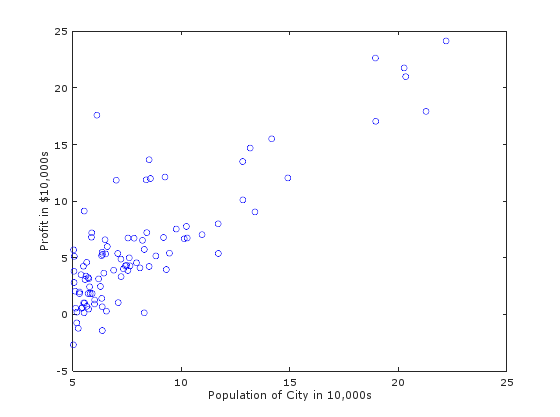
\includegraphics[width=0.42\textwidth]{03-bluecircles}
	\caption{Gráfica de círculos azules}
	\label{fig:bluecircles}
\end{figure}

\begin{figure}[h!]
	\centering
	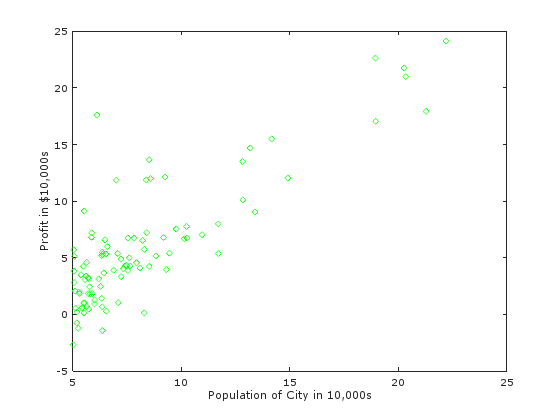
\includegraphics[width=0.42\textwidth]{03-greendiamonds}
	\caption{Gráfica de diamantes verdes}
	\label{fig:greendiamonds}
\end{figure}

\begin{figure}[h!]
	\centering
	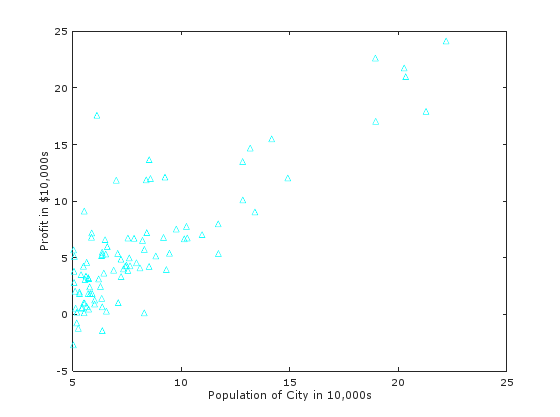
\includegraphics[width=0.42\textwidth]{03-cyantriangles}
	\caption{Gráfica de triángulos cian}
	\label{fig:cyantriangles}
\end{figure}

Posteriormente, se procedió a probar el algoritmo de descenso de gradiente.
Este algoritmo utiliza la función \texttt{computeCost} para evaluar la función mencionada en la Sección 2 de \texttt{ex1.pdf}.
Esta función es el cálculo del error cuadrático medio,
pero tiene una variante en donde la sumatoria del cuadrado de los errores es dividida entre $2n$.

El algoritmo encuentra los valores óptimos $\theta_i$,
que vienen a ser cada uno de los pesos del vector $w$, como se había visto en clase.
Los valores óptimos encontrados por el algoritmo son -3.630291 para $\theta_0$ y 1.166362 para $\theta_1$.

Después se agregó el criterio de regularización a la función de cálculo de costo en \texttt{computeCost.m},
utilizando un regularizador cuadrático, es decir, elevando la magnitud al cuadrado.
Para ello se probó con distintos valores de $\lambda$,
los cuales fueron 0, 0.01, 0.05, 0.5 y 1.

Las Figuras~\ref{fig:lambda005} y~\ref{fig:lambda001} muestran capturas de pantalla de los resultados para distintos valores de $\lambda$.

\begin{figure}[h]
	\centering
	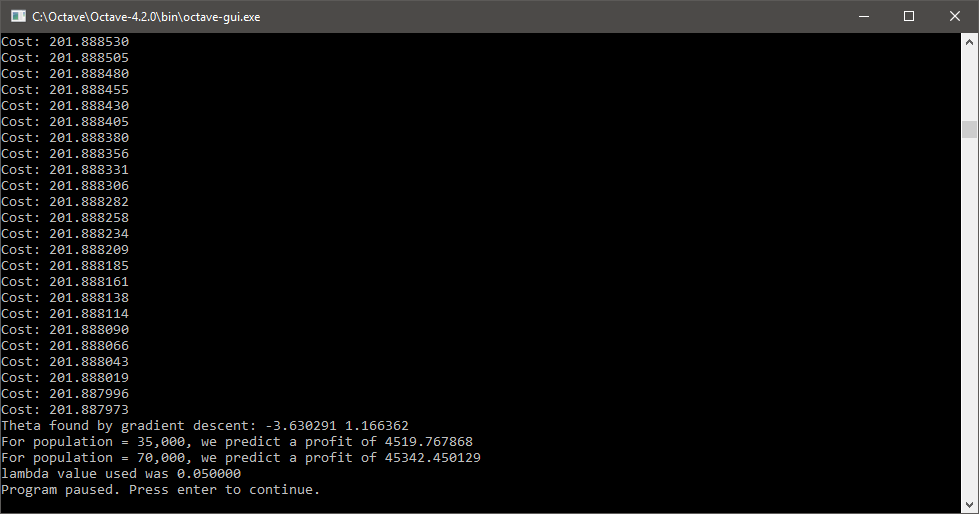
\includegraphics[width=0.95\textwidth]{03-lambda0dot05}
	\caption{Resultados para $\lambda=0.05$}
	\label{fig:lambda005}
\end{figure}

\begin{figure}[h!]
	\centering
	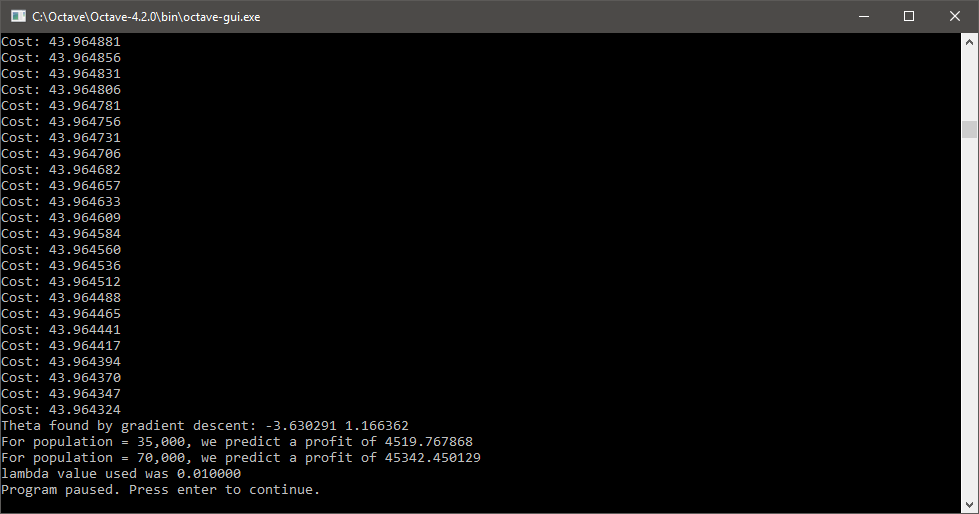
\includegraphics[width=0.95\textwidth]{03-lambda0dot01}
	\caption{Resultados para $\lambda=0.01$}
	\label{fig:lambda001}
\end{figure}

El resultado óptimo no cambió y tampoco las gráficas, por ende.
Sin embargo, se observó que el costo aumenta notoriamente al incluir el regularizador.
De esto se puede concluir que 1500 iteraciones,
que son las establecidas por defecto para el algoritmo de descenso de gradiente en el código provisto,
son demasiadas para el tamaño de la muestra: alrededor de 15 elementos.

% section ex1 (end)

\section{\textit{Deaths}, Tidy Data - Wickham} % (fold)
\label{sec:tidy}

La última parte del experimento fue recreada para la base de datos de mortalidad en México, provista en el repositorio mencionado en~\cite{JSSv059i10}, específicamente para los datos de la Figura 2.

Para ello, se agregó el criterio de regularización cuadrático con distintos valores de $\lambda$ al código del caso de estudio.
Al graficar los datos, almacenados en la variable \texttt{devi}, no se observó perturbación alguna por la suma del criterio de regularización para los valores de $\lambda$ utilizados;
tanto para la gráfica lineal como para la logarítmica.
Los valores de $\lambda$ son tan pequeños que el aumento no parece significativo.
% section tidy (end)

\section{Conclusiones y Reflexiones}
\label{sec:conc}

Este documento presentó una breve revisión de dos experimentos prácticos de aprendizaje supervisado.
A pesar de que se lograron analizar y contrastar algunos conceptos vistos en clase, es posible que haya habido errores humanos en el proceso de réplica por varias razones.
La primera de ellas es por el estándar de los datos.
Al ser archivos disponibles en diversos lugares de la red, las consultas pueden generar discrepancias por las diferentes versiones de los datos.
En segundo lugar, los errores de las réplicas podrían también deberse a que no existe estándar para comparación del producto final: ¿cómo se sabe que se está reportando y codificando la información correcta?
¿En qué dirección debería estar enfocado el reporte?
Estas preguntas surgen debido a las distintas interpretaciones que surgen al revisar las instrucciones.
Una revisión rápida a las instrucciones durante la clase sería de gran ayuda para casos donde pudiera existir ambigüedad.

Sin embargo, escribir el reporte y finalizar los experimentos ha representado un buen ejercicio de aprendizaje a nivel autodidacta.
Se generó un gran interés por el uso de \textit{Octave} para análisis matricial,
sobre todo porque puede llegar a ser muy útil para otras asignaturas.
Además, se generaron vínculos importantes con el resto de los compañeros de clase, pues en ocasiones atacar en equipo problemas de esta naturaleza es mucho más sencillo.


\bibliographystyle{IEEEtran}
\bibliography{IEEEabrv,02-biblio}

\end{document}